\secslide[\fontsize{1cm}{1cm}\selectfont]{Continuous Integration (CI),\\ Deployment,\\ and Continuous Delivery (CD)}

\begin{frame}[fragile]{What is Continuous Integration?}
  \begin{itemize}
    \setlength{\itemsep}{1em}
    \item A practice where tests and builds are run automatically, \eg, after code changes were
      merged/committed
    \item Goal: Find bugs, improve software quality (\eg, performance) and ensure
      your software runs on different platforms
    \item Every commit triggers a CI job
    \item Addressing failed CI jobs before merging a PR ensures code quality
    \item Running tests locally before committing adds an extra layer of ensuring code quality
  \end{itemize}
  \begin{block}{Note}
     The quality of your CI strongly depends on the quality of your tests.
     \begin{itemize}
      \item [\to] Requires effort beforehand.
     \end{itemize}
  \end{block}
\end{frame}


\begin{darkframe}[fragile]{CI: Multiple Platforms | GitHub Actions}
  \begin{enumerate}
        \begin{minted}{yaml}
          name: CI

          on:
            push:
              branches:
                - main
              tags:
                - '**'
            pull_request:

          env:
            MPLBACKEND: Agg
            PYTEST_ADDOPTS: --color=yes
        \end{minted}
  \end{enumerate}
\end{darkframe}

\begin{darkframe}[fragile]{CI: Multiple Platforms | GitHub Actions}
  \begin{enumerate}
    \setcounter{enumi}{1}
    \item We will be using GitHub Actions' matrix strategy to define multiple platforms:
        \scriptsize
        \begin{minted}{yaml}
          jobs:
            tests:
              runs-on: ${{ matrix.os }}
              strategy:
                matrix:
                  include:
                    - os: ubuntu-latest
                      python-version: "3.10"
                      install-method: mamba

                    - os: ubuntu-latest
                      python-version: "3.12"
                      install-method: mamba
                      extra-args: ["codecov"]  # lead platform for code cov

                    - os: ubuntu-latest
                      python-version: "3.12"
                      install-method: pip

                    - os: macos-13
                      python-version: "3.10"
                      install-method: pip

              defaults:
                run:
                  # We need login shells (-l) for micromamba to work.
                  shell: bash -leo pipefail {0}
        \end{minted}
  \end{enumerate}
\end{darkframe}

\begin{darkframe}[fragile]{CI: Multiple Platforms | GitHub Actions}
  \begin{enumerate}
    \setcounter{enumi}{2}
    \item Adding steps:
        \scriptsize
        \begin{minted}{yaml}
            steps:
              - uses: actions/checkout@v4
                with:
                  fetch-depth: 0

              - name: Prepare mamba installation
                if: matrix.install-method == 'mamba' &&  contains(github.event.pull_request.labels.*.name, 'documentation-only') == false
                env:
                  PYTHON_VERSION: ${{ matrix.python-version }}
                run: |
                  # setup correct python version
                  sed -i -e "s/- python=.*/- python=$PYTHON_VERSION/g" environment.yml

              - name: mamba setup
                if: matrix.install-method == 'mamba' && contains(github.event.pull_request.labels.*.name, 'documentation-only') == false
                uses: mamba-org/setup-micromamba@v1
                with:
                  environment-file: environment.yml
                  cache-downloads: true

              - name: Python setup
                if: matrix.install-method == 'pip' && contains(github.event.pull_request.labels.*.name, 'documentation-only') == false
                uses: actions/setup-python@v5
                with:
                  python-version: ${{ matrix.python-version }}
                  check-latest: true
        \end{minted}
  \end{enumerate}
\end{darkframe}

\begin{darkframe}[fragile]{CI: Multiple Platforms | GitHub Actions}
  \begin{enumerate}
    \setcounter{enumi}{3}
    \item For macOS, we have to fix the Python path:
        \scriptsize
        \begin{minted}{yaml}
          steps:
            - ...

            - if: matrix.install-method == 'pip' && runner.os == 'macOS' && contains(github.event.pull_request.labels.*.name, 'documentation-only') == false
              name: Fix Python PATH on macOS
              run: |
                tee -a ~/.bash_profile <<<'export PATH="$pythonLocation/bin:$PATH"'
        \end{minted}
  \end{enumerate}
\end{darkframe}

\begin{darkframe}[fragile]{
    Multiple Platforms | GitHub Actions
  }
  \begin{enumerate}
    \setcounter{enumi}{4}
    \item Install dependencies and run tests:
        \footnotesize
        \begin{minted}{yaml}
          steps:
            - ...

            - uses: astral-sh/setup-uv@v6

            - name: Install dependencies
              env:
                PYTHON_VERSION: ${{ matrix.python-version }}
              run: |
                python --version
                uv pip install --group tests -e .
                uv pip freeze
                uv pip list

            - name: List installed package versions (conda)
              if: matrix.environment-type == 'mamba'
              run: micromamba list

            - name: Tests
              run: |
                pytest -vv --cov --cov-report=xml

            - name: Upload coverage to Codecov
              uses: codecov/codecov-action@v4
              env:
                CODECOV_TOKEN: ${{ secrets.CODECOV_TOKEN }}  # make sure you have this set as repository secret
        \end{minted}
  \end{enumerate}
\end{darkframe}


\begin{darkframe}[fragile]{Codecov}
  \begin{enumerate}
    \item Sign up/log in to Codecov, \eg, via GitHub, GitLab, or Bitbucket
    \item Select your repository from your dashoard
    \item Select a setup option, \eg, \enquote{Using GitHub Actions}
    \item Select an upload token. For a single repository, the repository
      token is sufficient
    \item Add the token as repository secret
    \item Update your CI to automatically upload the coverage to Codecov (after the \texttt{Tests} step of your job)
      \begin{minted}{yaml}
        - name: Tests
          run: |
            pytest -vv --cov --cov-report=xml

        - name: Upload coverage to Codecov
          uses: codecov/codecov-action@v4
          env:
            CODECOV_TOKEN: ${{ secrets.CODECOV_TOKEN }}
      \end{minted}
  \end{enumerate}
  \vspace{0.25em}
  \begin{center}
    \huge\textcolor{cpink}{\to{} \textbf{NEVER} share your token with anyone.}
  \end{center}
\end{darkframe}


\begin{darkframe}[fragile]{Linting With the CI}
  \begin{center}
    
\includegraphics[height=3cm]{graphics/hank.jpg}\\[0.5\baselineskip]
    \huge\textcolor{ccyan}{%
      This is easier than ever: Set up your \texttt{.pre-commit-config.yaml},
      then go to \iref{pre-commit.ci/}{pre-commit.ci} and add your project/repository.
    }
  \end{center}
\end{darkframe}

\begin{darkframe}[fragile]{Building the Docs With the CI}
  The docs job can be started last.
  \footnotesize
    \begin{minted}{yaml}
      jobs:
        docs:
            runs-on: ubuntu-24.04
            steps:
              - uses: actions/checkout@v4
                with:
                  fetch-depth: 0

              - name: Set up Python
                uses: actions/setup-python@v5
                with:
                  python-version: "3.12"

              - name: Install doc dependencies
                run: |
                  sudo apt update -y && sudo apt install -y git build-essential pandoc graphviz ffmpeg
                  pip install -U pip towncrier setuptools
                  pip install -e .[docs]
                  git describe --tags

              - name: Build docs
                run: make -C docs html
    \end{minted}
\end{darkframe}

\begin{darkframe}{CI/CD: DevOps}
  \begin{center}
    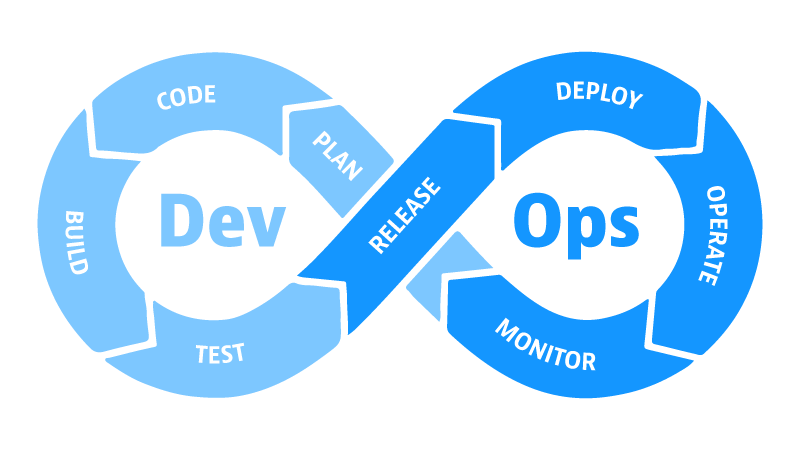
\includegraphics[height=0.6\textheight]{graphics/devops.png}
  \end{center}
\end{darkframe}

\begin{darkframe}[fragile]{CD: Publish on PyPI}
  \begin{minted}{yaml}
    name: Build Python Package

    on:
      push:
      workflow_dispatch:
      release:
        types:
          - published

    jobs:
      dist:
        runs-on: ubuntu-latest
        steps:
          - uses: actions/checkout@v4
          - uses: hynek/build-and-inspect-python-package@v2
            with:
              path: .
  \end{minted}
\end{darkframe}

\begin{darkframe}{CD: Publish on PyPI (cont.)}
  \begin{minted}{yaml}
    jobs:
      distlong:
        runs-on: ubuntu-latest
        steps:
          - uses: actions/checkout@v4
            with:
              fetch-depth: 0

          - uses: astral-sh/setup-uv@v6

          - name: Build SDist and wheel
            run: uvx --from build pyproject-build

          - uses: actions/upload-artifact@v4
            with:
              name: Packages-distlong-${{ github.job }}
              path: dist/*

          - name: Check metadata
            run: uvx twine check ./dist/*
  \end{minted}
\end{darkframe}

\begin{darkframe}{CD: Publish on PyPI (cont.)}
  \begin{minted}{yaml}
    jobs:
      publishtrusted:
        needs: [ dist ]
        environment: pypi
        permissions:
          id-token: write
          attestations: write
          contents: read
        runs-on: ubuntu-latest
        if: github.event_name == 'release' && github.event.action == 'published'
        steps:
          - uses: actions/download-artifact@v4
            with:
              name: Packages
              path: dist

          - name: Generate artifact attestation for sdist and wheel
            uses: actions/attest-build-provenance@v2
            with:
              subject-path: "./dist/*"

          - uses: pypa/gh-action-pypi-publish@release/v1
  \end{minted}
\end{darkframe}

\begin{frame}{Further Reading: CI/CD}
  \begin{columns}[t,onlytextwidth]
    \begin{column}{0.48\textwidth}
      \begin{itemize}
        \setlength{\itemsep}{1em}
        \item \iref{https://docs.google.com/presentation/d/1em_YjW-KcbQZLbNVL5izIJHiBxeMOq7GsSilcDoDIx0/}{Jonas Eschle's PYOPP Talk}
        \item \iref{https://indico.desy.de/event/43817/sessions/19712/attachments/97983/135044/docs_ci_pyopp_2025.pdf}{My PYOPP Talk}
        \item \iref{https://docs.github.com/en/actions}{GitHub Actions}
        \item \iref{https://github.com/actions/checkout}{actions/checkout}
        \item \iref{https://github.com/astral-sh/setup-uv}{astral-sh/setup-uv}
        \item \iref{https://github.com/mamba-org/setup-micromamba}{setup-micromamba}
      \end{itemize}
    \end{column}
    \begin{column}{0.48\textwidth}
      \begin{itemize}
        \setlength{\itemsep}{1em}
        \item \iref{https://docs.codecov.com/docs/}{Codecov}
        \item \iref{https://docs.github.com/en/actions/writing-workflows/choosing-what-your-workflow-does/running-variations-of-jobs-in-a-workflow}{Matrix Strategies}
        \item \iref{https://pre-commit.ci/}{pre-commit.ci}
        \item \iref{https://docs.gitlab.com/ci/}{GitLab CI}
        \item \iref{https://docs.gitlab.com/ci/variables/predefined_variables/}{GitLab: Predefined Variables}
        \item \iref{https://badge.fury.io/}{badge.fury.io} and \iref{https://shields.io/}{shields.io} (Badges)
      \end{itemize}
    \end{column}
  \end{columns}
\end{frame}
